\documentclass[aps,prl,preprint,superscriptaddress]{revtex4-1}

\usepackage{graphicx}
\usepackage{amsmath}
\usepackage{hyperref}

\usepackage{listings}
\usepackage{xcolor}
\lstdefinestyle{pythonstyle}{
  language=Python,
  basicstyle=\ttfamily\small,
  keywordstyle=\color{blue},
  stringstyle=\color{red},
  commentstyle=\color{gray},
  breaklines=true,
  numbers=left,
  numberstyle=\tiny\color{gray},
  stepnumber=1,
  numbersep=5pt,
  aboveskip=0pt,
  belowskip=0pt,
  lineskip=-0.5ex,
}
\lstset{style=pythonstyle}

\begin{document}

    % Titulo y Abstracto
    \title{Situación Problema Entregable Final}

\author{Facundo Bautista Barbera}
\email{a01066843@tec.mx}
\affiliation{Escuela de Ingeniería y Ciencias, campus Monterrey.\\ Tecnológico de Monterrey}

\author{Luis Santiago Vargas Ochoa}
\email{a01563708@tec.mx}
\affiliation{Escuela de Ingeniería y Ciencias, campus Monterrey.\\ Tecnológico de Monterrey}

\date{\today}
    \begin{abstract}

    En este reporte se presentan los resultados de la experimentación realizada con un método de compresión de imágenes basado en la Transformada Discreta de Fourier en dos dimensiones (FFT 2D). Se introduce el problema y se explica la elección de la FFT 2D como ténica ce compresión. En la sección de exprimentación se detalla el flujo de trabajo implmentado en Python. Finalmente, se hace una comparación de las tasas de compresión obtenidas en imágenes a color y en escala de grisis.

\end{abstract}

    \maketitle

    % Intoducción
    \section{Introducción}

En esta segunda entrega de la situación problema para la unidad de formación de Análisis Métodos Matemáticos Para La Física,
se presentan los resultados de la investigación realizada en la primera etapa y los resultados de experimentación de compresión de imágenes.

Dando un poco de contexto adicional, hoy en día, enormes volúmenes de imágenes son generados y compartidos a diario, desde fotografías personales hasta imágenes satelitales o médicas.
La compresión de imágenes es un proceso útil para poder disminuir el espacio de almacenamiento necesario para manejar este tipo de datos no estructurados. 
Un archivo de imagen sin comprimir (con algún formato de tipo RAW) almacena la información píxel por píxel y suele tener un tamaño considerable. 

Utilizando métodos de compresión es posible reducir de forma impactante el tamaño de un archivo de imagen, logrando mantener una calidad visual aceptable. Un formato popular es el formato JPEG, el cual logra tasas de compresión cercanas al 90\% (Es decir, comprime la imagen a un 10\% de su tamaño original), manteniendo una calidad de imagen considerable.
Esto se logra gracias a la redundancia de información visual y las limitaciones de percepción que tiene el ojo humano.

Existen dos tipos principales de compresión: sin pérdida (lossless), donde la imagen original se puede reconstruir exactamente igual, y con pérdida, donde se permite una leve degradación a cambio de mayores tasas de compresión.
Para las experimentaciones realizadas para esta situación problema, se probará crear un script que cree una compresión con pérdida.

    \newpage
    % Experimentación
    \section{Experimentación}

\subsection{Entorno y herramientas}

El proceso de experimentación se desarrolló usando Python 3.12, usando un entorno virtual (venv) para poder reproducir el proyecto facilmente. Para el computo numérico y las trasnformadas se uso NumPy (v2.3.0). La lectura y escritura de imágenes utiliza Pillow (v11.2.1) para formatos estándar y rawpy (v0.25.0) para archivos RAW@.

\subsection{Proceso de compresión}

En esta sección se busca descrbir el flujo completo de compresión.
Se implementa en una clase \texttt{Image}, definida en \texttt{image.py}, integrando la parte programática y matemática.

\subsubsection{Carga de la imagen}

Se abre un archivo (RAW, JPEG, u otros tipos) usando Pillow o rawpy, en caso de que la imagen sea de tipo RAW y se convierte en un array de NumPy de tipo Float.

\begin{lstlisting}[language=Python, caption={Método \_load\_image}, label={lst:load_image}]
def _load_image(self, image_path, greyscale=False):
    try:
        img = PILImage.open(image_path)
    except (UnidentifiedImageError, OSError):
        with rawpy.imread(image_path) as raw:
            rgb = raw.postprocess(no_auto_bright=True, output_bps=8)
            img = PILImage.fromarray(rgb)
    img = img.convert('L' if greyscale else 'RGB')
    return np.array(img, dtype=float)
\end{lstlisting}

\subsubsection{Transformada de Fourier en 2D}

Se aplica la FFT bidimensional y centramos el espectro para revelar las compontentes de frecuencia (se usa numpy para estos procesos).

\begin{lstlisting}[language=Python, caption={Método \_fast\_fourier\_transform}, label={lst:fft2d}]
def _fast_fourier_transform(self, image_array):
    ft = np.fft.fft2(image_array, axes=(0,1))
    return np.fft.fftshift(ft)
\end{lstlisting}

La FFT 2D parte de la idea de la FFT 1D, la cual normalmente se usa para descomponer señales unidimensionales en una suma de ondas sinusoidales de distintas freuencias y amplitudes. En este caso nuestra `onda` es una función bidimensional \(f(x,y)\) que corresponde a la imagen.
La FFT 2D procesa filas y columnas simultáneamente y genera un mapa bidimensional de las frecuencias horizontales y verticales.

\newpage

\subsubsection{Enmascaramiento del espectro}

\begin{lstlisting}[language=Python, caption={Enmascaramiento del espectro}, label={lst:masking}]
magnitude = np.abs(fourier_transformed)
threshold = np.percentile(magnitude, 100 * (1 - ratio))
mask = magnitude > threshold
fourier_compressed = fourier_transformed * mask
\end{lstlisting}

Al aplicar un umbral sobre las magnitudes de este espectro, conservamos únicamente los componentes más importantes. Este umbral se calibró con un ratio de pérdida de 0.1, lo que significa que se descarta hasta el 90\% de las características menos relevantes durante la compresión, sin afectar significativamente la calidad visual.

\subsubsection{Transformada inversa}

\begin{lstlisting}[language=Python, caption={Transformada inversa}, label={lst:inverse_transform}]
img_back = np.fft.ifft2(np.fft.ifftshift(fourier_compressed)).real
img_back = np.clip(img_back, 0, 255).astype(np.uint8)
\end{lstlisting}

Se reconstruye la imagen utilizando IFFT2D, es decir la transformada inversa despues de haber recortado los valores fuera de rango.

\subsubsection{Guardado del resultado}

\begin{lstlisting}[language=Python, caption={Guardado de la imagen comprimida}, label={lst:save_image}]
img = PILImage.fromarray(img_back)
img.save(output_path, quality=100, subsampling=0)
\end{lstlisting}

Se utiliza Pillow para exportar la imagen comprimida con calidad máxima, evitando pérdidas adicionales de compresión.


    \newpage
    % Comparación
    \section{Comparación}

Para poder ilustrar mejor las diferencias entre las imágenes originales y las comprimidas, tanto en escala de grises como en color, se creó un notebook de Jupyter que presenta los resultados visuales. Esta notebook fue generada con apoyo de herramientas con inteligencia artificial y cumple únicamente el propósito de demostración gráfico y no afecta directamente en el desarrollo técnico de proyecto.

\subsection{Imagenes de comparación}

\begin{figure}[htbp]
  \centering
  \includegraphics[width=0.8\textwidth]{sources/comparison/test_1.png}
  \caption{Resultados de compresión imagen 1}\label{fig:comparison1}
\end{figure}

\begin{figure}[htbp]
  \centering
  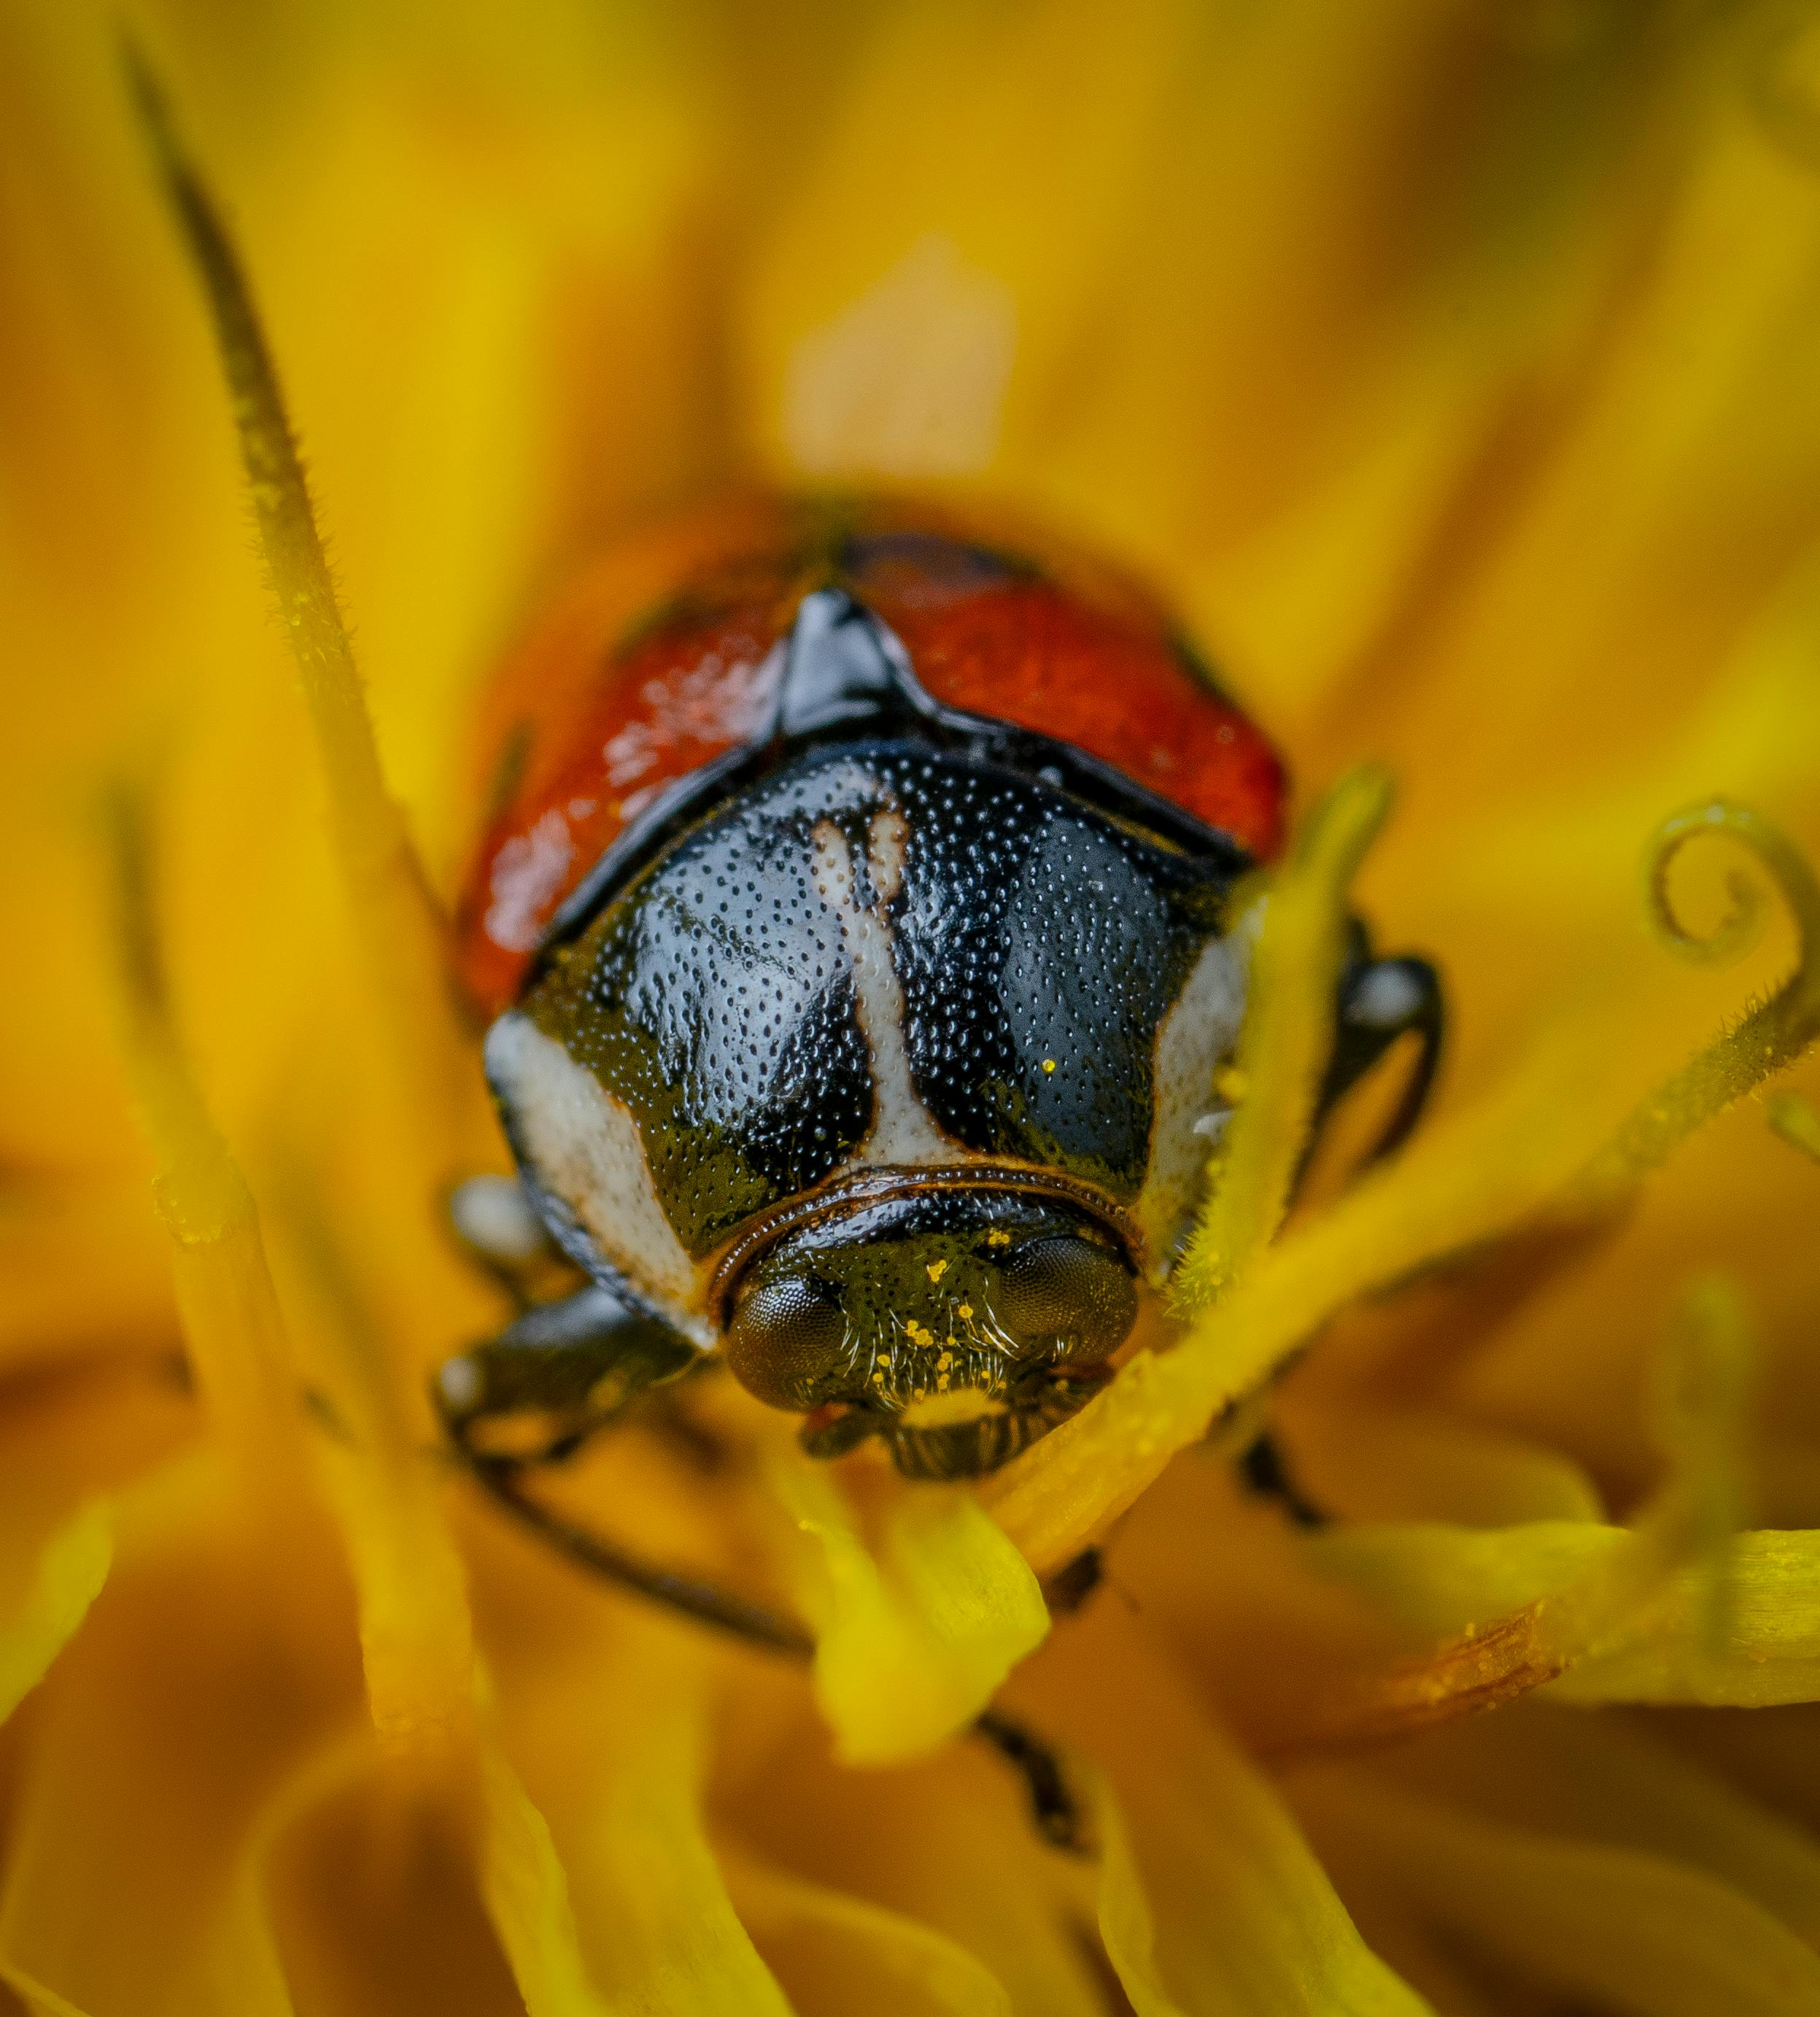
\includegraphics[width=0.8\textwidth]{sources/comparison/test_2.png}
  \caption{Resultados de compresión imagen 2}\label{fig:comparison2}
\end{figure}

\begin{figure}[htbp]
  \centering
  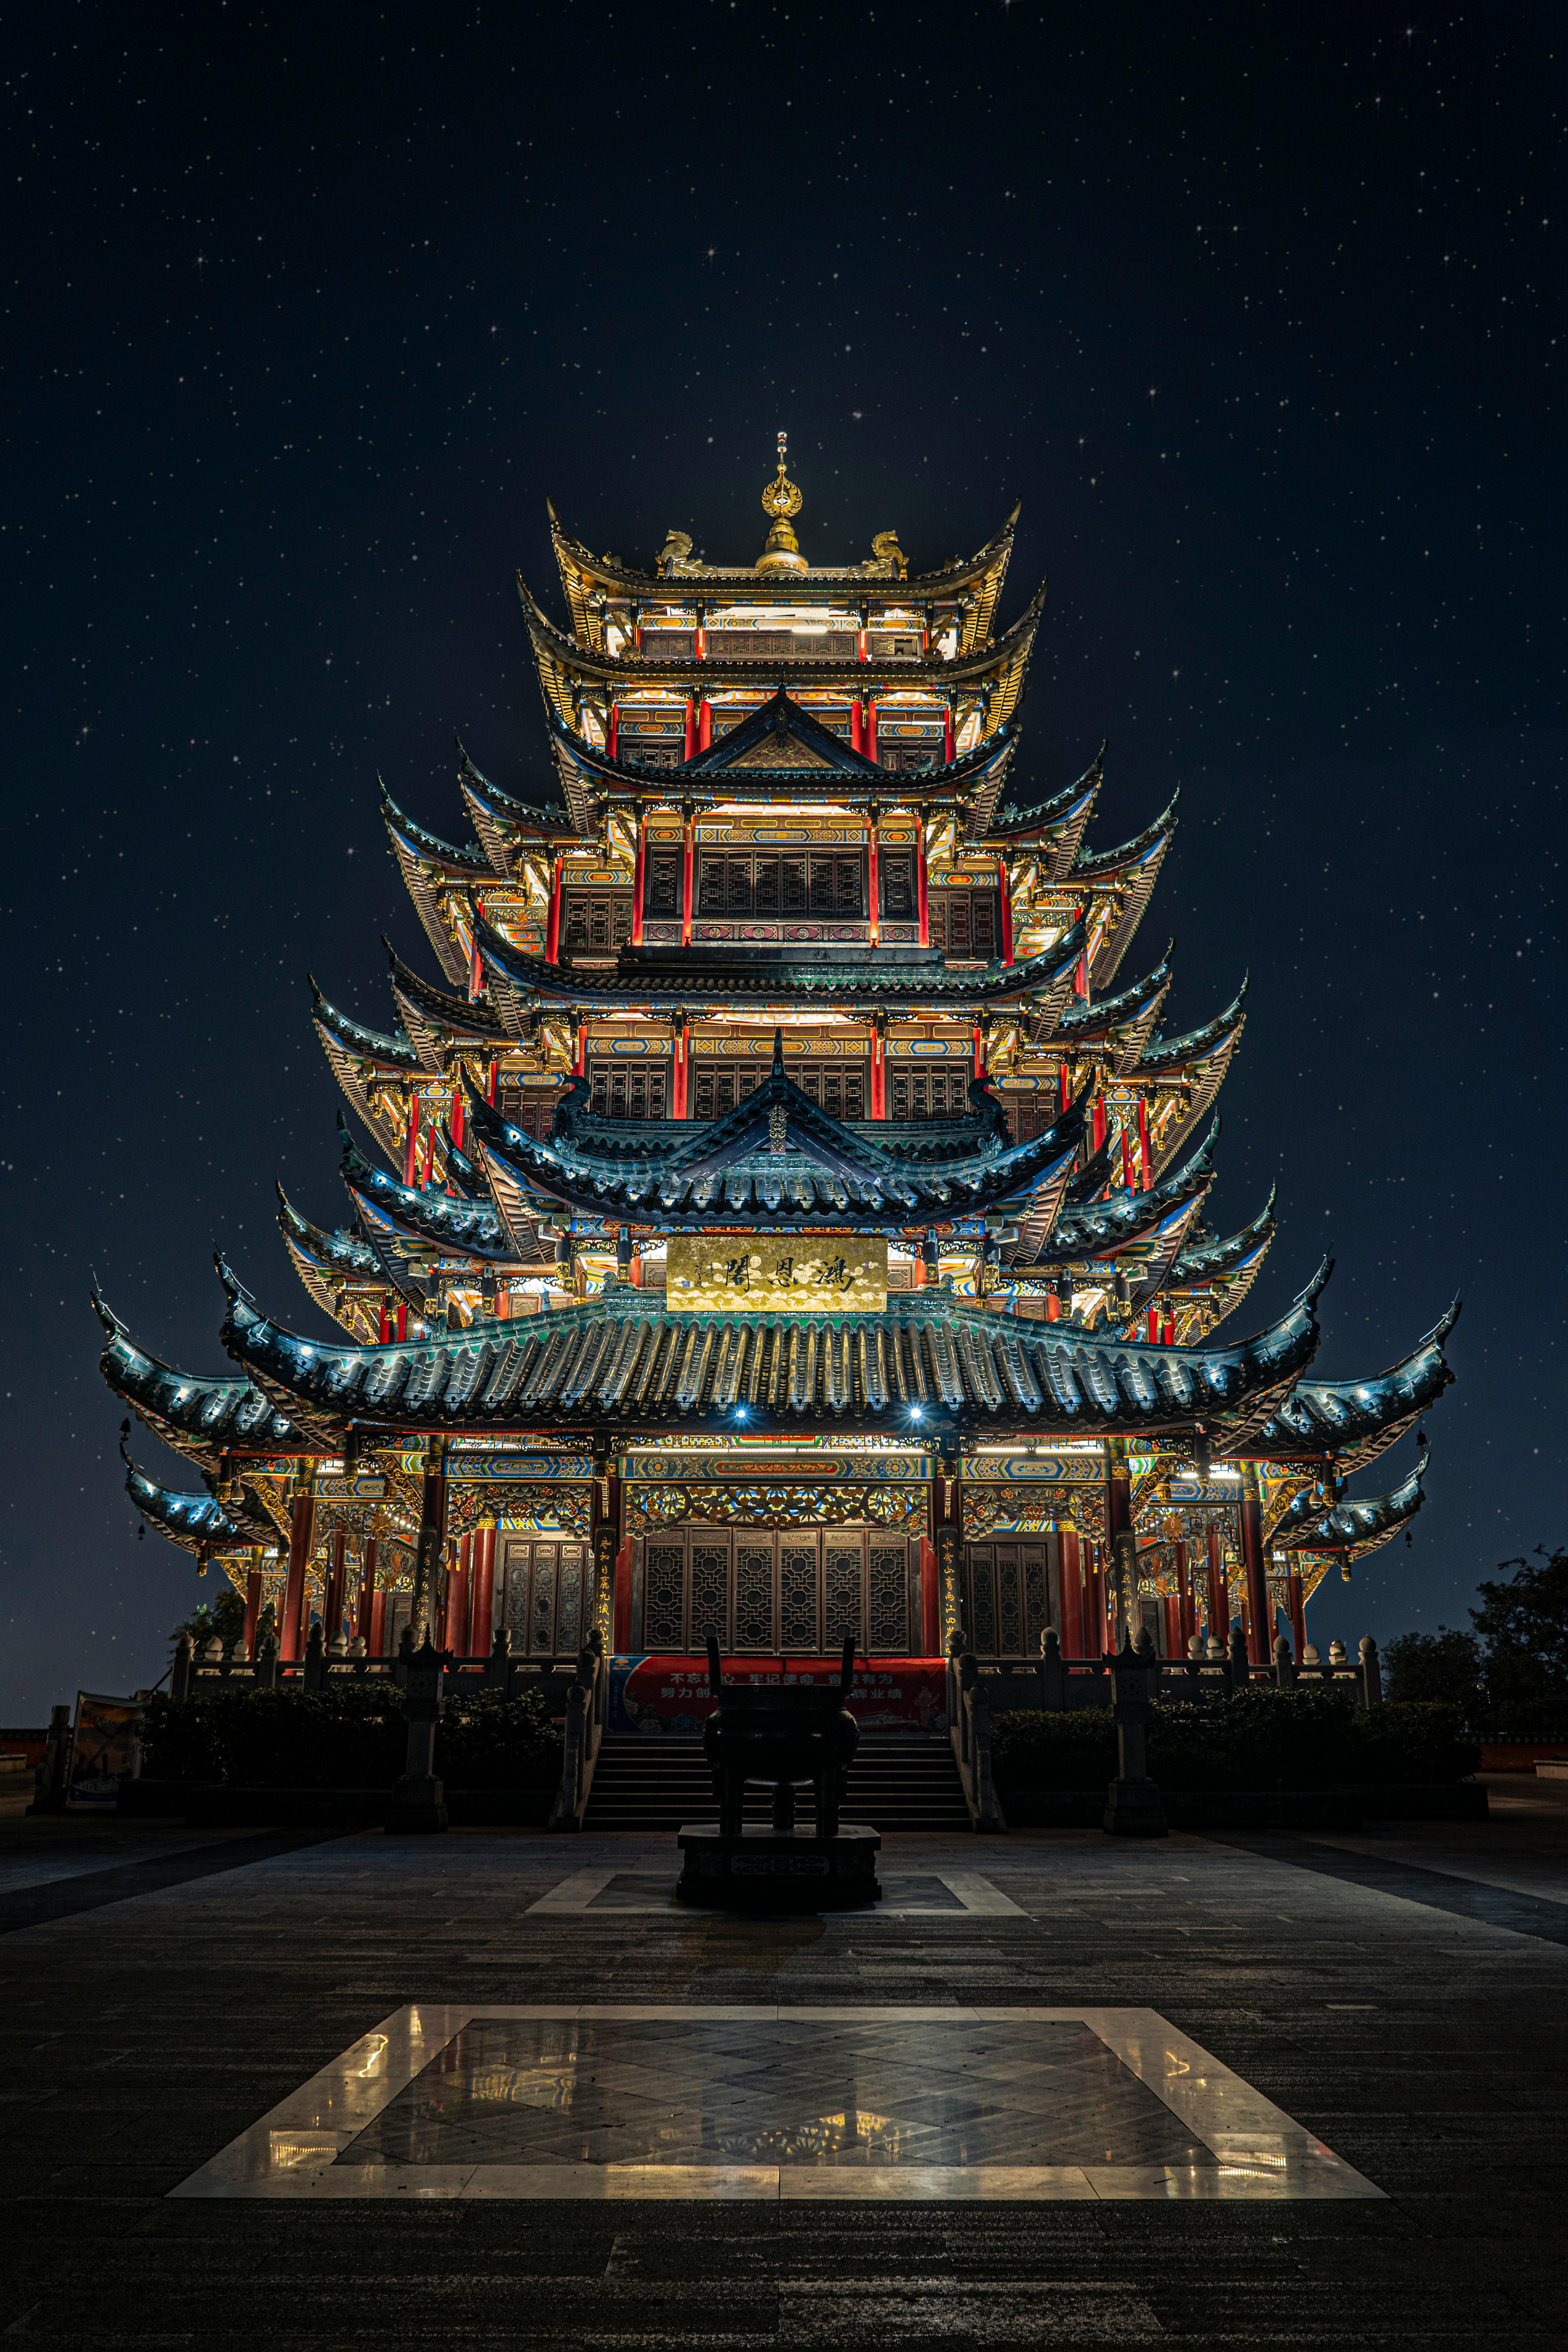
\includegraphics[width=0.8\textwidth]{sources/comparison/test_3.png}
  \caption{Resultados de compresión imagen 3}\label{fig:comparison3}
\end{figure}

\subsection{Observaciones sobre las imagenes}

Con la implementación del método basado en FFT 2D se logró reducir el tamaño de los archivos sin sacrificar visualmente los detalles esenciales. Al transformar las imágenes se mantiene intacta una estructura general, contornos, gradaciones suaves y las texturas continuas.

Para las imágenes de color, el método FFT 2D logra reducir las imágenes entre un 50\% y un 60\% de su tamaño original. Esto se debe a que los 3 canales de color (rojo, verde y azul) comparten redundancias y el FFT 2D logra descartar muchas frecuencias sin que aparezca perceptibles.

Para las imágenes en escala de grises se puede observar que la compresión es menor, se logra reducir entre un 15\% y un 25\%, lo cual sigue siendo un tamaño considerable.

Visualmente se puede observar que las imágenes son perfectamente perceptibles. Al ampliar la imagen comprimida, se puede percibir una ligera cantidad de ruido y algunos bordes ligeramente más duros, pero cumple con la función de compresión.

Es importante destacar que aunque la compresión es consistente en la mayor parte de los casos, aunque si existe la posibilidad de que la imagen no se comprima adecuadamente si esta contiene muchos detalles granulares o ruido visual (como partículas).

    \newpage
    % Conclusiones
    \section{Conclusiones}

Este reporte presentó un método de compresión de imágenes con base en la Transformada Discreta de Fourier en dos dimensiones (FFT 2D). Los resultados de la experimentación demuestran que la técnica implementada permite alcanzar tasas de compresión considerables, lo cual es aún más notable en imágenes comprimidas con color, gracias a las redundancias de los canales cromáticos. A pesar de la eficiencia que tiene el modelo, este también puede tener sus limitaciones, como producir ruido visible en zonas con mucho detalles o texturas granuladas, y un umbral fijo no adapta automáticamente a variaciones locales de contenido (es decir, ajuste de enmascaramiento por región de imagen).

\subsection{Nota de Facundo}

Considero que este reporte y, en general, el proceso de experimentación fue bastante satisfactorio.
El desarrollar el código que implementa un método matemático para hacer algo real y útil fue realmente entretenido. Aplicar las transformadas de Fourier para algo que no sea simplemente resolver un problema matemático cualquiera realmente ayuda a centrar más la utilidad del concepto. Desde un inicio me pareció increíble como es que las series y transformada de Fourier logran capturar elementos `escondidos`' en las cosas y creo que este conocimiento me será realmente útil en el futuro para entender cosas como redes neuronales.

    \newpage
    % Referencias
    \section{Referencias}

    \nocite{*}
    \bibliographystyle{apsrev4-2}
    \bibliography{sources/references}

    \newpage
    \appendix
    
    \section{Anexo: Código Python}
    \lstinputlisting[caption={Código de compresión de imagen en Python},label={lst:imagecompression}]{../src/image.py}

    \newpage
    \lstinputlisting[caption={Código para procesar todas las imagenes},label={lst:imagecompressionstartup}]{../compress_all.py}

\end{document}